\documentclass{article}
\usepackage[utf8]{inputenc}
\usepackage{enumitem}
\usepackage{graphicx}
\usepackage{amssymb}
\usepackage{hyperref}
\graphicspath{{./notepics/}}
\hypersetup{colorlinks=true, urlcolor=blue}
% swnat = start w/ name and today
\newcommand{\swnat}[1]{\begin{document} \begin{flushleft} Date of notes: \today \\ #1 \\}
\newcommand{\iit}{\item}
\newcommand{\iitsub}[1]{\begin{itemize} \item{#1} \end{itemize}}
\newcommand{\mathline}[1]{\vspace*{0.75em}\centerline{#1}}
\newcommand{\fancyL}{$\mathcal{L}$}
\newcommand{\fancydeltaL}{$\nabla \mathcal{L}$}
\newcommand{\fancyR}{$\mathbb{R}$}
\newcommand{\la}{$\leftarrow$ }
\newcommand{\ra}{$\rightarrow$ }
\newcommand{\setin}{$\in$ }
\newcommand{\firstitemstart}[1]{\section*{#1 Notes} \begin{itemize}[leftmargin=*] \setlength\itemsep{.005em}}
\newcommand{\restitemstart}[1]{\end{itemize} \section*{#1 Notes} \begin{itemize}[leftmargin=*] \setlength\itemsep{.005em}}
% note: can't make a newcommand w/ 'end' 
\newcommand{\docitemend}{\end{itemize} \end{flushleft} \end{document}}
\swnat{CAP 4600 All Notes}
\firstitemstart{1.a. Slide}
\iit In terms of being a superset, AI \ra Machine learning \ra Deep learning.
\iit Symbolic AI (also called GOFAI): term for collection of all methods in AI based in symbolic representation.
\iit Diagram of above: input \& rules \ra [machine] \ra output.
\iit ML programs adjust themselves in response to data they're exposed to.
\iit ML is dynamic and doesn't require human intervention to make certain changes.
\iit Diagram of ML: input \& output \ra [machine] \ra rules.
\restitemstart{1.b. Slide}
\iit ML has paradigms, mostly either through supervised or unsupervised learning.
\iit Supervised learning: ML where model is provided w/ labeled training data.
\iit Features and their corresponding labels are fed into an algorithm in the training process.
\iit The algorithm gradually determines the relationship btw. features and corresponding labels, called a model.
\iit Finding patterns btw. data and labels in supervised ML learning can be expressed mathematically as functions.
\iit Unsupervised learning: identifying meaningful patterns in data (and using that to understand the importance of new data).
\iit Reinforcment learning: at time step $t$, the agent is in state $s_t$, takes action $a_t$, receives reward 
$r_t$, and transitions into state $s_{t+1}$.
\iit Agent has to learn which actions to take at the current state for the maximum rewards.
\iit You also need to provide a way for the agent to interact w/ the game to produce data, physically or virtually.
\restitemstart{2.a. Slide}
\iit Supervised ML learning terminology:
\iit Label: what we seek to predict.
\iit Feature $x_j$: input variable that is used to predict the label, where $j \in \{1,\ldots, n\}$ where $n$ is the number of features.
\iit Many features can be used for projects requesting more regulation.
\iit Example: particular instance of data fed into models
\iit Labeled ex.: includes both features and the label, like: \{features, label\}: (x,y)
\iitsub{Used to train model.}
\iit Unlabeled ex.: only features, like: \{features, ?\}: (x,?)
\iitsub{We use the model once it's done training w/ labeled examples to predict the label on unlabeled examples.}
\iit Training: creating or learning the model.
\iitsub{Show the model $(x,y)$ such that it can learn the relationships btw. feature $x$ and 
label $y$ such that prediction $\hat{y}$ is sufficiently close to the label $y$.}
\iit Inference: means applying the trained model to unlabeled examples (making useful predictions $\hat{y}$)
\iit Regression model: predicts continuous vals. (numerical)
\iit Classification model: predicts discrete vals. (descriptive)
\restitemstart{2.b. Slide}
\iit Linear regression: finding the relationship of data through the formula $y=mx+b$
\iit ML equation is slightly different w/ $\hat{y}=b+w_1 x_1$, where:
\iitsub{$\hat{y}$: predictied label (desired output), $b$ is the bias (y-int.) [also called $w_o$], 
$w_1$ is the weight of feature 1 [weight is similar to slope $m$], and $x_1$ is a feature (known input).}
\iit To infer (predict) $\hat{y}$ for a new val. $x_1$, just substitute $x_1$ val. into this model.
\iitsub{Bigger models would rely on multiple features $x_1, x_2, \ldots, x_n$, each having seperete weights $w_1, w_2, \ldots, w_n$.
\iitsub{For example: a model w/ three features might look like: 
$\hat{y}=b+w_1 x_1+w_2 x_2+w_3 x_3 = b + \sum^{3}_{j=1} w_j x_j$. }}
\restitemstart{2.c. Slide}
\iit Training: examining the examples and adjusting the weights \& bias so that the loss is minimized.
\iit Loss: penalty for a bad prediction, quantifying how bad the model's prediction was on a single example.
\iit The goal of training: finding a set of weights \& biases that have low loss across 
all examples on average (process called empirical risk minimization).
\iit Use of a square loss employed as a loss function (also known as a $L_2$ loss).
\iitsub{If we let $w = (b, w_1, \ldots, w_n)$ be the params. of the model (weights and bias), 
and features be w/ $x = (x_1, \ldots, x_n)$ label $y$, the model will predict $\hat{y} = f_w(x) = b + \sum^{n}_{j=1} w_j x_j. $
\iitsub{The squared loss for a single example the difference btw. label (obs.) $y$ and prediction $\hat{y}$: $(y-\hat{y})^2$.}}
\iit Mean square error (MSE): average squared loss per example over whole dataset:
$MSE(w) = 1/m \sum^{m}_{i=1} (y^{(i)} - \hat{y}^{(i)})^2$.
\iitsub{$m$ is the number of examples, $x^{(i)} = (x_1^{(i)}, \ldots, x_n^{(i)})$ \& $y^{(i)}$ are the features 
and the label of the $i$th example, and $\hat{y}^{(i)}$ is the prediction of the model.
\iitsub{Formally, $\hat{y} = f_w(x^{(i)}) = b + \sum^{n}_{j=1} w_j x_j^{(i)}. $}
Although MSE is heavily used in ML, it isn't the best loss function or the the only practical loss function for every circumstance.}
\restitemstart{2.d. Slide}
\iit Iterative learning: try to reduce loss iteratively (guess a val. of $w_1$ and wait for the system to tell us what the loss is)
\iit If we adapt the weights correctly, we will be decreasing the loss over time. 
The challenge is to find the best possible model as efficiently as possible.
\iitsub{The iterative trial-and-error process that ML algos. use to train a model includes: \\
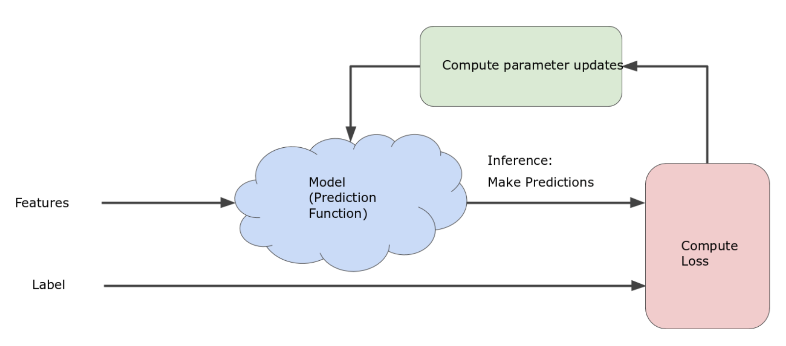
\includegraphics[scale=0.5]{iterative} \centering}
\iit Iterative strats. are prevalent in ML because they scale so well to large data sets. The model takes features $x_1, \ldots, x_n$
as input and returns one prediction $\hat{y}$ as output. 
\iitsub{ If we consider that the simplest lin. reg. model that takes only one feature as input: $\hat{y} = b + w_1 x_1$. 
For lin. reg. problems, we can pick random vals. for the starting positions $b$ \& $w_1$. }
% note: double qoutes must look like {``} for the first part and {''} for the last part
\iit If we look inside the ``Compute parameter updates'' part of the diagram, we can see the ML system examines the val. of the loss function
\& generates new vals. for $b$ \& $w_1$. We can say for now that it devises new vals. \& then the ML system re-evaluates all those features
against all those labels, yielding a new val. for the loss function, which yields new param. values. The learning continues iterating until the ML system discovers the model params. w/ the lowest possible loss. Usually, we iterate until the loss stops changing or at least there are extremely slow changes to the model. If this happenes, we can say the model has converged.
\iit A ML model is trained by starting w/ an init. guess for the weights \& bias and iteratively adjusting those guesses until finding
the weights \& the bias w/ the lowest possible (or sufficiently low) loss are found.
\restitemstart{2.e. Slide}
\iit Gradient descent algo.: When we consider the linear regression model $\hat{y}=f_w(x) = b+w_1 x_1+w_2 x_2+ \ldots + w_n x_n$,
where $w=(w_0, w_1, \ldots, w_n)$, The loss function (MSE): \\ 
\centerline{\fancyL$ $ : \fancyR $^{n+1}$ \ra \fancyR} 
depends on the params. $n+1$ params. $b, w_1, \ldots, w_n$. The loss is given by: \\
\mathline{\fancyL$ $ = $1/m \sum^{m}_{i=1} 1/2(\hat{y}^{(i)} - y^{(i)})^2$}
\mathline{$= 1/m \sum^{m}_{i=1} 1/2(f_w(x^{(i)}-y^{(i)}))^2$}
\mathline{$= 1/m \sum^{m}_{i=1} 1/2(\sum^{n}_{j=1} w_j x_j + b - y^{(i)})^2.$}
\vspace*{-0.125em}\iit For $n=1$, the loss function \fancyL$ $ depends on two params., the bias term $b = w_0$ and the weight $w_1$, \& defines a surface in 3D. For $n > 1$, the loss function \fancyL$ $ cannot be visualized easily. To simplify the plots, we assume that $n = 1$ and the bias term $b = w_0$ is fixed to be 0. Then the loss function \fancyL$ $ depends only on $w_1$ and defines a curve. 
\iit The resulting plot of the loss function \fancyL$ $ is convex (assuming graph is loss over value of weight $w_1$). Even in the general case, the loss function \fancyL$ $ is convex. This is important since problems only have one min. 
Calculating the loss function for all param. values $w_0, \ldots, w_n$ \setin \fancyR $^{n+1}$ would be an inefficient way of finding the min.
Let's examine a better mechanism (very pop. in ML) called gradient descent.
\iit The starting point doesn't matter in the first stage in gradient descent, so we can set $w_i = 0$ or a rand. val.
\iit The gradient descent algo. then calculates the gradient of the loss function \fancyL$ $ at the starting point. The gradient 
\fancydeltaL\setin\fancyR$^{n+1}$ is a vector whose entries $($\fancydeltaL$)_i$ are given by the partial derivs. $\partial$\fancyL$/ \partial w_i$
of the loss function \fancyL$ $ with respect to the weights $w_i$.
\iit The \fancydeltaL$ $ gradient has both a dir. and a mag. 
The graident points which way is closer or farther from the intended target.
The gradient always points in the dir. of steepest increase in the loss function. For the case $n=1$ \& the bias $w_0 = b$ is fixed to be 0, the gradient of the loss function \fancyL $ $ is simply the slope of the curve \fancyL$ $, that is, the deriv. w/ respect to $w_1$. 
\iitsub{The gradient descent algo. takes a step in the direction of the negative gradient $-$\fancydeltaL$ $ to reduce the loss. 
More precisely, the gradient descent algo. updates the starting point as follows: w \la w $- \alpha$\fancydeltaL, where $\alpha$ is the learning rate.}
\iit The gradient vector also has both a dir. \& a mag. The gradient descent algo. multiplies the grad. by a scalar known as the learning rate
(also sometimes called step size) to determine the next point. The learning rate is a so-called hyperparameter: a parameter that is external
to the model.
\iitsub{If the learning rate is too small, learning will take too long, but if it is too large, the next point will perpetually bounce haphazardly
across the bottom of the well. There must be a Goldilocks learning rate for every linear reg. problem.}
\restitemstart{\href{https://colab.research.google.com/drive/1CdwvzRhFNIlhp1mWVWFXSXAsmRFWvASq}{Python3}}
\iit Primitive Datatypes -- straighforward
\iit Control Statements (if, for, while, etc.) -- remember to add ``:'' after statements and to indent
\restitemstart{\href{https://colab.research.google.com/drive/1eECClMU1r-Y9hzPnRw89__jC3nw3C-zD}{Effect of Learning Rate on Gradient Descent for Finding Minima of Univariate Functions}}
\iit Notebook for experimenting with different learning rates and understanding what could go wrong when applying gradient descent with a poorly chosen learning rate.
\iit Overstepping in the learning rate could have massive consequences, while also getting stuck in a local minimum could stall the progress of the ML process.
\docitemend
